
\subsubsection{International Patent Classification code}
In 1971, the Strasbourg Agreement established the International Patent Classification (IPC) under the World Intellectual Property Organization (WIPO), which divides technology into eight discrete Sections. The goal of this
Agreement was to overcome the difficulties caused by using diverse national patent classification systems.~\citep{harris2010comparison}

A patent is assigned to one or more of the 71,000 IPC codes that 
indicate the related technical field or fields the patent covers. 
These codes are arranged in a hierarchical, tree-like structure with 
five distinct components. Fig. \ref{fig:ipcexample} illustrates the components of an IPC classification.

The highest hierarchical level contains the eight sections of the IPC corresponding
to very broad technical fields, labeled A through H. For example, Section C deals
with``Chemistry and Metallurgy''. Sections are subdivided into classes. The eighth edition of the IPC contains 120
classes. Class C07, for example, deals with ``Organic Chemistry''. Classes are further subdivided into more than 600 subclasses. Subclass C07C, for example, deals with ``Acyclic or Carbocyclic Compounds''. Subclasses are then further divided into main groups and subgroups. Main group symbols end with ``/00''. Ten percent of all IPC groups are main
groups. For example, main group C07C 35/00 deals with ``Compounds having at
least one hydroxy or O-metal group bound to a carbon atom of a ring other than
a six-membered aromatic ring''. In some versions of the IPC, a series of numbers will follow the subgroup, reflecting
the enactment date of the IPC version. `20060101' following the Subgroup
indicates a date of January 1, 2006, which is the date that the eighth version of
the IPC took effect. 
%%%%%%%%%%%%%%%%%%%%%%%%%%%%%%%%%%%%%%%%%%%%%%%%%%%%%%%%%%%%%%%%%%%%%%%%%%%%%%%%%
\begin{figure}[t!]
   \centering
   \includegraphics[width=0.70\textwidth,height=35mm]{figs/IPCexample.jpg}
   \caption{An example illustrating the components of an International Patent Classification code.}   
   \label{fig:ipcexample} 
\end{figure}
%%%%%%%%%%%%%%%%%%%%%%%%%%%%%%%%%%%%%%%%%%%%%%%%%%%%%%%%%%%%%%%%%%%%%%%%%%%%%%%%%
%\subsubsection{IPC Classification as a Filter}
\subsubsection{International Patent Classification Code as a Filter}
IPC code has been recommended by previous works as a filter in retrieval process. By applying the IPC code filtering, the system ignores the documents which has no similar IPC code with the patent query. 

In this experiment, we investigate weather all relevant patent documents have at least one IPC code common with the patent query for three different level of hierarchy. 
\paragraph{(I) Filter: 4-digit IPC code}
\ \\
First, we investigate the effect of four digits of IPC code as a filter, which includes `Section', `Class', and `Subclass'. 
This is the filter we are using for our system. 
%For the false negative patents (complete patents in English), 
The results show that about 19\% of not retrieved relevant patents do not share any IPC code with the patent query, but the majority of them have query main IPC code, and about 21\% share, at least, one of the query further IPC codes (Fig. \ref{fig:fnipcoverlap}). 
%%%%%%%%%%%%%%%%%%%%%%%%%%%%%%%%%%%%%%%%%%%%%%%%%%%%%%%%%%%%%%%%%%%%%%%%%%%%%%%%%
\begin{figure}[t!]
   \centering
   \includegraphics[width=0.60\textwidth,height=69mm]{figs/ipcOverlap-FNs.png}
   \caption{Classification code overlap between the query and non-relevant retrieved patents (False Negative (FN) patents).}   
   \label{fig:fnipcoverlap} 
\end{figure}
%%%%%%%%%%%%%%%%%%%%%%%%%%%%%%%%%%%%%%%%%%%%%%%%%%%%%%%%%%%%%%%%%%%%%%%%%%%%%%%%%
%%%%%%%%%%%%%%%%%%%%%%%%%%%%%%%%%%%%%%%%%%%%%%%%%%%%%%%%%%%%%%
%\begin{figure}[t!]
%\begin{centering}
%\subfigure[Cut-off rank(k) = 100\label{fig:datacuration_a}]{\includegraphics[width=6.5cm]{figs/ipcOverlap-FNs.png}}  
%\subfigure[Cut-off rank(k) = 1000\label{fig:datacuration_b}]{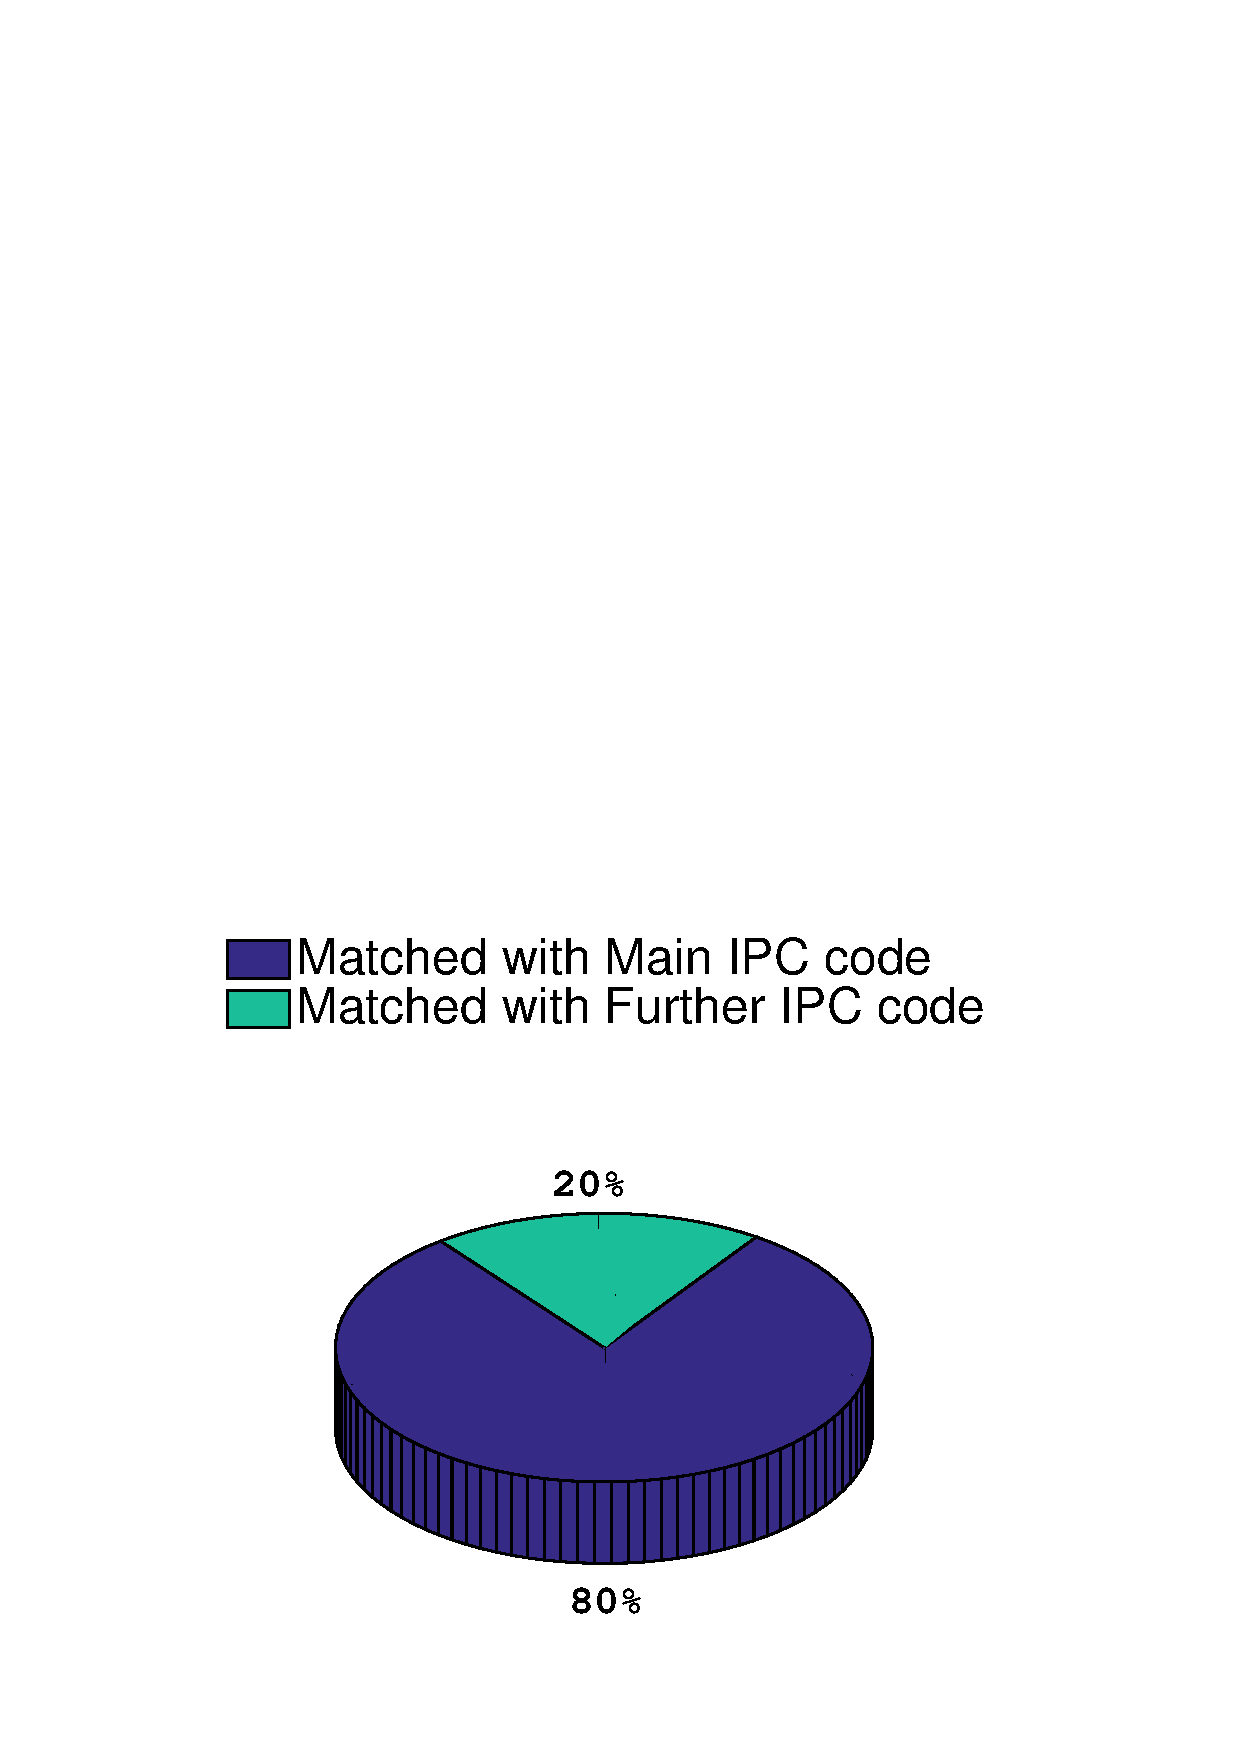
\includegraphics[width=6.5cm]{figs/ipcOverlap-TPs.png}} 
%\par\end{centering} 
%\protect\caption{Average percentage of errors due to missing `Description', non-English original language. Overall, 37\% of errors are because of data curation while 63\% of English complete patent documents can not be retrieved. Increasing k from 100 to 1000 reduces the errors of red area, but 42\% is still notable.}
%\label{fig:datacuration}
%\end{figure}
%%%%%%%%%%%%%%%%%%%%%%%%%%%%%%%%%%%%%%%%%%%%%%%%%%%%%%%%%%%%%%

On the other hand, as it has been shown in Figure \ref{fig:tpipcoverlap} all TP patents have 80\% overlap with the main query IPC code and 20\% with, at least, one of the query further IPC codes. 
%So, we can conclude that 19\% of errors can be due to IPC filtering if we assume that they have enough term overlap with the query.  
%%%%%%%%%%%%%%%%%%%%%%%%%%%%%%%%%%%%%%%%%%%%%%%%%%%%%%%%%%%%%%%%%%%%%%%%%%%%%%%%%
\begin{figure}[t!]
   \centering
   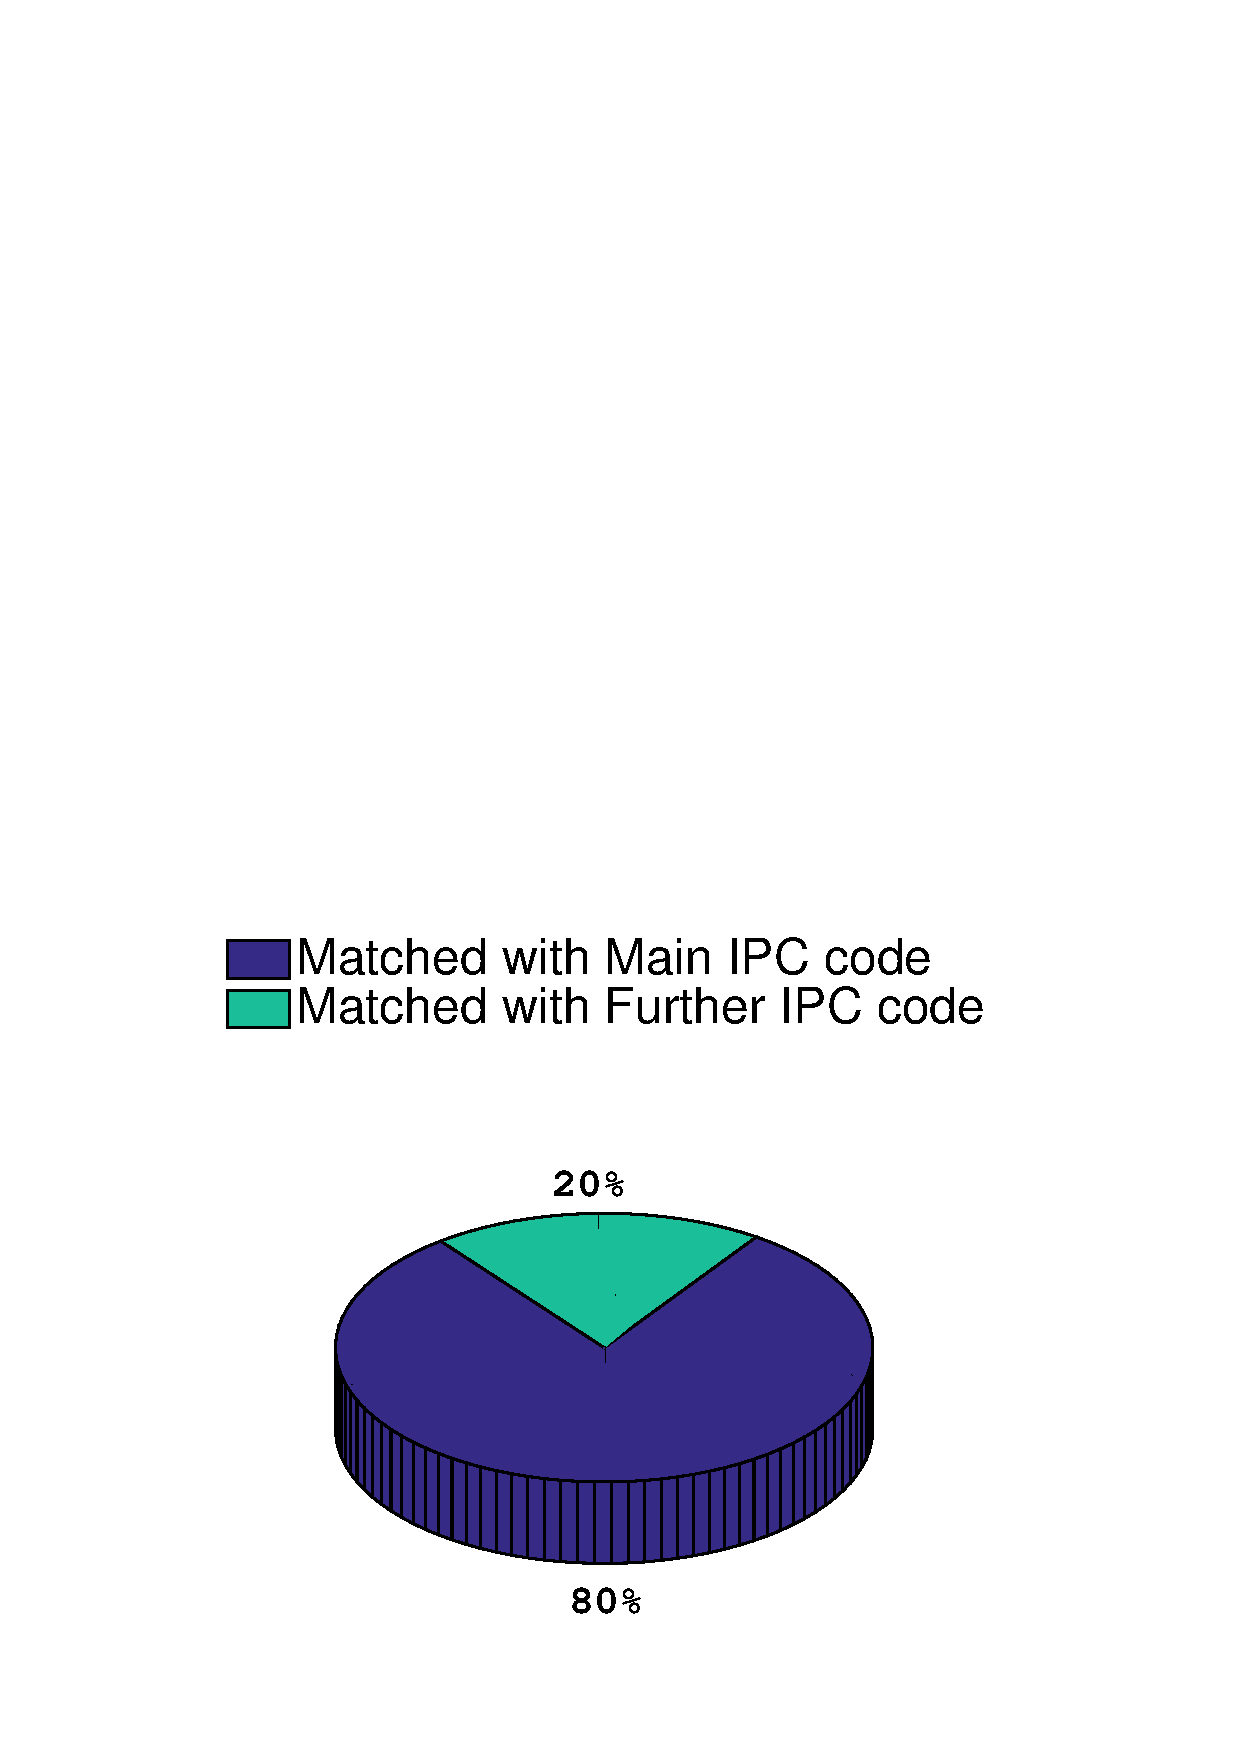
\includegraphics[width=0.55\textwidth,height=60mm]{figs/ipcOverlap-TPs.png}
   \caption{Classification code overlap between the query and relevant retrieved patents (True Positive (TP) patents).}   
   \label{fig:tpipcoverlap} 
\end{figure}
%%%%%%%%%%%%%%%%%%%%%%%%%%%%%%%%%%%%%%%%%%%%%%%%%%%%%%%%%%%%%%%%%%%%%%%%%%%%%%%%%
Using 4-digit IPC code filter causes 19\% of the errors, however, we still keep the filter on in our experiments, because of two main reasons: 
\begin{enumerate}
\item CLEF-IP 2010 collection contains 2.6 million patent documents. If we set the filter: \textit{off}, it will be time consuming to match the query to the whole collection. However, by applying the filter, this process will be done faster and instead of the whole collection, matching process is done on the portion of the collection which share an IPC code with the patent query. Since less than 19\% of errors are due to classification mismatch, we continue our analysis by keeping the filter: \textit{on} because the matching process is computationally much faster compared to what we lose by applying the IPC filter. The computational time is critical in patent prior-art search as the query is the `Description' of the the patent query, which contains thousands of words.   
\item Precision in the top k=100 drops significantly when ranking the whole collection versus the portion that have shared classification code with the query.  
\end{enumerate}
To justify the first reason, in the following experiment, we calculate the number of documents which have at least one of the query IPC code. In average, this number is `$ 36254 $', which indicates, in average for each query, the system just needs to look into `$ 36254 $' documents instead of the entire collection containing 2.6 million patent documents. Therefore, keeping the IPC filter: \textit{on}, we will computationally save lots of time.  
%%%%%%%%%%%%%%%%%%%%%%%%%%%%%%%%%%%%%%%%%%%%%%%%%%%%%%%%%%%%%%%%%%%%%%%%%%%%%%%%%
\begin{figure}[t!]
   \centering
   \includegraphics[width=0.70\textwidth,height=68mm]{figs/ipcfilter-histo.png}
   \caption{The distribution of the number of patents should be ranked for each query over all test queries(1303), after applying the IPC filter: 4-digit IPC code.\\
In average, the matching process for each query is done over  `$ 36254 $' documents instead of the whole collection(2.6 million documents) which reduce the computational time dramatically.}   
   \label{fig:ipcfilter-histo} 
\end{figure}
%%%%%%%%%%%%%%%%%%%%%%%%%%%%%%%%%%%%%%%%%%%%%%%%%%%%%%%%%%%%%%%%%%%%%%%%%%%%%%%%%
%\FloatBarrier 
%\noindent

Figure~\ref{fig:ipcfilter-histo} shows the distribution of documents should be processed against each query after applying IPC filter. It indicates that by applying the IPC filter, we reduce the computation time by reducing the number of documents to be processed from the whole collection to `$ 36254 $' documents, in average. In trade off between losing 19\% of relevant patents and making the ranking process quicker, we chose the faster computation. The histogram falls down by increasing the number of documents that should be processed; This means that the majority of queries need to do matching process with less documents. 
%\vspace{-1cm}
\paragraph{(II) Filter: First two components of the IPC code}
%\textbf{(B) Filter: First two components of the IPC code}
\ \\
Our baseline system applying the first 4-digit IPC code as a default(e.g. C07C in Figure~\ref{fig:ipcexample}), including `section', `class', and `subclass'. One way to reduce the error related to IPC code filtering is to broaden the filter by selecting two first components of the query IPC (e.g. C07). The result of making the filter broader has been plotted in Figures~\ref{fig:ipc1stTwoElements} and~\ref{fig:firstTwoIpcFilter-histo}. Figure~\ref{fig:ipc1stTwoElements} shows that we can reduce the error related to filtering from 19\% to 13\% by omitting the subclass component. However, as it can be seen in Figure~\ref{fig:firstTwoIpcFilter-histo}, the number of documents that should be processed during ranking increased to `$ 99754 $' in average. 
%%%%%%%%%%%%%%%%%%%%%%%%%%%%%%%%%%%%%%%%%%%%%%%%%%%%%%%%%%%%%%%%%%%%%%%%%%%%%%%%%
\begin{figure}[t!]
   \centering
   \includegraphics[width=0.55\textwidth,height=60mm]{figs/ipc1stTwoElements.png}
   \caption{Filter: The first two components (Section and Class).}   
   \label{fig:ipc1stTwoElements} 
\end{figure}
%%%%%%%%%%%%%%%%%%%%%%%%%%%%%%%%%%%%%%%%%%%%%%%%%%%%%%%%%%%%%%%%%%%%%%%%%%%%%%%%%
%\FloatBarrier 
%\noindent
%\vspace{-1em}

%\begin{figure}[htpb]
%\centering
%\begin{subfigure}[htpb]{.5\linewidth}
%\centering
%\includegraphics[width=1\textwidth,height=55mm]{figs/ipc1stTwoElements.png}
%\caption{Filter: The first two components (Section and Class)}
%\label{fig:ipc1stTwoElements}
%\end{subfigure}%\\[1ex]%
%\begin{subfigure}[htpb]{.5\linewidth}
%\centering
%\includegraphics[width=1\textwidth,height=55mm]{figs/ipc1stElement.png}
%\caption{Filter: Only the first component (Section)}
%\label{fig:ipc1stElement}
%\end{subfigure}
%\caption{IPC classification overlap between the query and the FN patents after making the filter broader.}
%\label{fig:restrictedipc}
%\end{figure}
%\FloatBarrier
%%%%%%%%%%%%%%%%%%%%%%%%%%%%%%%%%%%%%%%%%%%%%%%%%%%%%%%%%%%%%%%%%%%%%%%%%%%%%%%%%
\begin{figure}[t!]
   \centering
   \includegraphics[width=0.70\textwidth,height=68mm]{figs/firstTwoIpcFilter-histo.png}
   \caption{The distribution of the number of patents should be ranked for each query over all test queries (1303).
In average, the matching process for each query is done over `$ 99754 $' documents instead of the whole collection (2.6 million documents) which reduce the computational time dramatically.}   
   \label{fig:firstTwoIpcFilter-histo} 
\end{figure}
%%%%%%%%%%%%%%%%%%%%%%%%%%%%%%%%%%%%%%%%%%%%%%%%%%%%%%%%%%%%%%%%%%%%%%%%%%%%%%%%%
%\FloatBarrier 
%\vspace{-5em}
%\noindent
\paragraph{(III) Filter: First component of the IPC code}
%\textbf{(C) Filter: First component of the IPC code}
\ \\
 We can even make the filter less restrict by choosing only the first component (e.g. C), corresponding to very technical fields. If we use just the first IPC component (`Section') as a filter, there would still be 7\% error due to IPC mismatch between the query and relevant documents (Figure~\ref{fig:ipc1stElements}). 
%\vspace{-1em}
%%%%%%%%%%%%%%%%%%%%%%%%%%%%%%%%%%%%%%%%%%%%%%%%%%%%%%%%%%%%%%%%%%%%%%%%%%%%%%%%%
\begin{figure}[t!]
   \centering
   \includegraphics[width=0.50\textwidth,height=55mm]{figs/ipc1stElement.png}
   \caption{Filter: Only the first component (Section).}   
   \label{fig:ipc1stElements} 
\end{figure}
%%%%%%%%%%%%%%%%%%%%%%%%%%%%%%%%%%%%%%%%%%%%%%%%%%%%%%%%%%%%%%%%%%%%%%%%%%%%%%%%%

Figure~\ref{fig:firstIpcFilter-histo} shows the distribution of the number of patents should be ranked for each query over all test queries (1303), after applying the IPC filter
%: ``\textit{only the first component of the IPC code}". 
In average, the matching process for each query is done over `$ 415828 $' documents instead of the whole collection(2.6 million documents). This number is much higher than using more restricted filters and will not be efficient computationally. 
%The min number of documents considered during matching process is `$ min=41721 $', and the maximum is `$ max=1058447 $'. 

The results show that using only the first component of the IPC code is not appropriate because it can not reduce the computational time as well as there is still 7\% error.   
%\vspace{-2em}
%%%%%%%%%%%%%%%%%%%%%%%%%%%%%%%%%%%%%%%%%%%%%%%%%%%%%%%%%%%%%%%%%%%%%%%%%%%%%%%%%
\begin{figure}[t!]
   \centering
   \includegraphics[width=0.60\textwidth,height=60mm]{figs/firstIpcFilter-histo.png}
   \caption{The distribution of the number of patents should be ranked for a query over all test queries (1303), after applying the IPC filter: ``\textit{only the first component of the IPC code}".
In average, the matching process for each query is done over `$ 415828 $' documents instead of the whole collection (2.6 million documents). This number is much higher than using more restricted filters and will not be efficient computationally. 
%The min number of documents considered during matching process is `$ min=41721 $', and the maximum is `$ max=1058447 $'
}   
   \label{fig:firstIpcFilter-histo} 
\end{figure}
%%%%%%%%%%%%%%%%%%%%%%%%%%%%%%%%%%%%%%%%%%%%%%%%%%%%%%%%%%%%%%%%%%%%%%%%%%%%%%%%%

In conclusion, errors related to IPC code mismatch with the query is quite acceptable in trade-off with the computational benefit we gain using IPC code filter. Among all three kind of filters we applied, using 4-digit IPC code has been computationally the most effective. Since, it reduce the ranking process to be done over $ 36254 $ documents in average instead of the whole collection. Two other filters are not computationally as efficient as the 4-digit IPC code filter. Furthermore, there is still error even if we make the filter more broad.
